\documentclass[a4paper, landscape]{article}

%\geometry{showframe}% for debugging purposes -- displays the margins

\usepackage{savetrees}

\usepackage{amsmath}
\usepackage{amssymb}
\usepackage{color}
\usepackage{hyperref}
\usepackage{colortbl}
\usepackage[normalem]{ulem}

\usepackage{tikz}
\usetikzlibrary{shapes.multipart}

\usepackage{fancyvrb}

<< pygments['pastie.tex'] >>

\setlength{\parindent}{0pt}
\setlength{\parskip}{1ex plus 0.5ex minus 0.2ex}

\begin{document}

\section{Overview by Portfolio}

<% for portfolio in f.portfolios() -%>

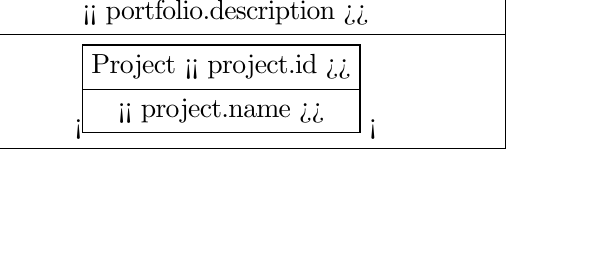
\begin{tikzpicture}[
double/.style={draw, anchor=text, rectangle split,rectangle split parts=2},
triple/.style={draw, anchor=text, rectangle split,rectangle split parts=3}
]

\node[draw, anchor=text, rectangle split,rectangle split parts=3] {Portfolio << portfolio.id >> : << portfolio.name >>
    \nodepart{second}
    << portfolio.description >>
    \nodepart{third}
    <% for project in portfolio.projects() -%>
    \tikz{\node[double] { Project << project.id >> \nodepart{second}<< project.name >>};}
    <% endfor -%>
};
\end{tikzpicture}

<% endfor -%>

\newpage

<% for portfolio in f.portfolios() -%>

Portfolio << portfolio.id >> : << portfolio.name >>

<< portfolio.description >>

\begin{itemize}
<% for recipe in portfolio.recipes() -%>
\item{Recipe << recipe.id >> : << recipe.name >>}
<% endfor -%>
\end{itemize}

\begin{itemize}
<% for project in portfolio.projects() -%>
\item{Project << project.id >> : << project.name >>}
<% endfor -%>
\end{itemize}

<% endfor -%>

\newpage
\section{Overview by Project}

<% for project in f.projects() -%>
<< project.portfolio().name >> - Project << project.id >>: << project.name >>

\begin{itemize}
<% for note in project.notes() -%>
\item{Note << note.id >>) << note.note >>}
<% endfor -%>
\end{itemize}


\begin{itemize}
<% for task in project.tasks() -%>
\item{<% if task.completed_at -%>\sout{<% endif -%><< "~~~" * (project.indent() + task.indent() + 1) >><< task.display_line() >><% if task.completed_at -%>}<% endif -%>}
<% endfor -%>
\end{itemize}


<% endfor -%>

\newpage
\section{Task View}

\begin{tabular*}{\textwidth}{|l|c|l|l|}
\hline
<% for task in f.tasks() -%>
<% if task.waiting_for_task_id -%>
\rowcolor[gray]{0.5}
% Could also put \color commands in each cell to color the text, would be better for printing.
<% endif -%>
<< task.id >> & << task.context >> & << task.due() >> & << task.name >> \\
        \hline
<% endfor -%>
\end{tabular*}

\newpage
\section{Notes}

<% for note in f.inbox_notes() -%>
Note << note.id >>. << note.note >>
<% endfor -%>

\end{document}
